\documentclass[]{article}
\usepackage[utf8x]{inputenc}
\usepackage{graphicx}
\usepackage{hyperref}
\usepackage[english,italian]{babel}
\begin{document}

\title{Proposta Tirocinio e Tesi Triennale:\\Drone quadricottero}
\author{Stefano Radaelli, matricola 869863}
\maketitle

\section{Scopo del Tirocinio}
Lo scopo di questo tirocinio non è quello di inventare un nuovo oggetto partendo da un'idea innovativa, ma quello di applicare le nozioni imparate nel corso di questi anni per la realizzazione di un progetto, seppure già esistente.\\Intendo, quindi, fare uno studio sugli algoritmi e sulle leggi fisiche e matematiche che permettano la realizzazione di un prodotto informatico che, dovendo volare, dev'essere anche capace di interagire con agenti esterni (quali gravità, attrito, vento, pressione ecc...).\\ Tramite questo studio algoritmico e fisico sarà possibile trovare la migliore tecnica di volo stabile, applicata ad un drone quadricottero. La bontà di stabilità di volo può essere poi misurata tenendo conto di quanto il drone riuscirà a sembrare "fermo" in volo, come nel seguente video: \\
\url{https://www.youtube.com/watch?v=w2itwFJCgFQ}\\ Questo video rappresenta, secondo me, la massima stabilità in volo raggiungibile, a cui potrò ispirarmi.

\section{Obiettivi}
L'obiettivo principale è quello di creare un drone quadricottero (quattro motori) funzionante e stabile in volo. La stabilità in volo sarà ottenuta grazie al bilanciamento dei motori tramite l'ausilio di sensori come giroscopio e accelerometro. Inizialmente, il drone potrà essere comandato tramite un sistema di controllo a distanza, come un trasmettitore "radiocomando" a 2.4Ghz. L'aspetto più importante di un drone è che, in assenza di input esterno, esso dev'essere in grado di mantenere la quota in volo, e quindi non cadere ("stabilize" o "hovering"). 
Una volta raggiunti questi requisiti necessari per il funzionamento base, potranno essere implementate altre funzionalità, quali:
\begin{itemize}
\item Altitude Hold: Il drone mantiene un'altezza costante in assenza di input.
\item Loiter: In assenza di input, il drone mantiene la sua esatta posizione grazie all'ausilio di un GPS.
\item Auto: Il drone segue un percorso prestabilito.
\item Altro.
\end{itemize}
Il raggiungimento dell'obiettivo principale necessiterà però di uno studio approfondito sulla dinamica di volo e sul funzionamento di ogni singolo componente da utilizzare. La parte più difficile sarà sicuramente la calibrazione dei motori, per permettere un volo preciso senza barcollamento. Il giroscopio dovrà essere posizionato al centro esatto del drone, ovvero il punto meno affetto da vibrazioni, mentre l'algoritmo a livello software dovrà fare in modo che il drone si trovi il più possibile parallelo al terreno durante il volo. Un altro studio interessante può essere il comportamento del drone in caso di batteria quasi scarica durante il volo, come ad esempio l'atterraggio automatico. 
Ovviamente, considero per ora gli aspetti e difficoltà derivanti solo dal funzionamento base, e non dagli upgrade successivi, che necessiteranno di ulteriori studi.

\section{Funzionamento Principale}
Il drone, essendo quadricottero, avrà 4 motori collegati ad eliche, accoppiati in diagonale, due che girano in senso orario e due in senso antiorario (Figura 1). Il drone, per sollevarsi in volo, dovrà produrre una forza verticale (portanza) che si opponga alla forza peso. Ciò avviene grazie ad una differenza di pressione generata dall'elica. Il drone, quindi, potrà eseguire spostamenti grazie alla differenza di forza verticale generata dalle diverse eliche. Ad esempio, per spostarsi in avanti, la forza generata dalle eliche posteriori dev'essere maggiore della forza generata da quelle anteriori.
\begin{figure}[!htpb]
\centering
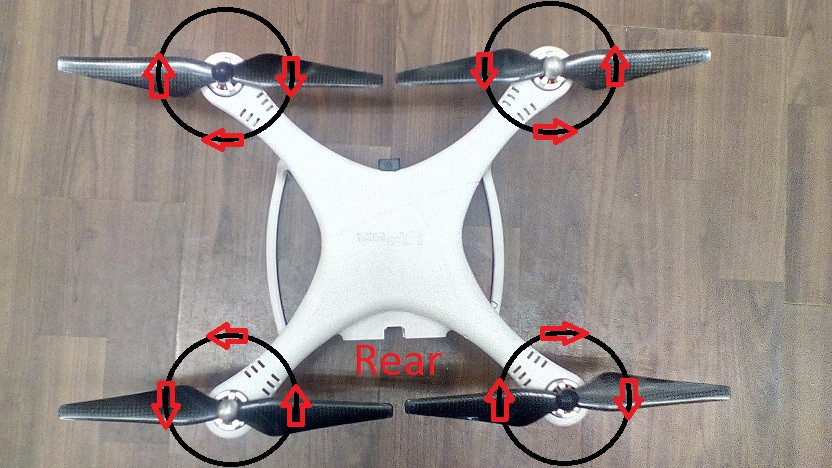
\includegraphics[scale=0.3]{figura1.jpg}
\caption{Motori}
\label{figura1}
\end{figure}
\section{Hardware (per funzionamento base)}
L'hardware necessario potrà essere comprato singolarmente(Amazon, dx.com ecc...) oppure recuperato da droni preassemblati (da cui recuperare telaio e motori). Non escludo la possibilità di comprare un drone nuovo realmente funzionante per poi smontarlo.
Oltre, ovviamente, ad una board Embedded (da definire), sono previsti i seguenti componenti;
\subsection{Telaio}
Il telaio (Figura 2) è la struttura portante del drone. Dev'essere abbastanza leggero da poter permettere il volo. I materiali più utilizzati per droni entry level sono plastica o alluminio.
\begin{figure}[!htpb]
\centering
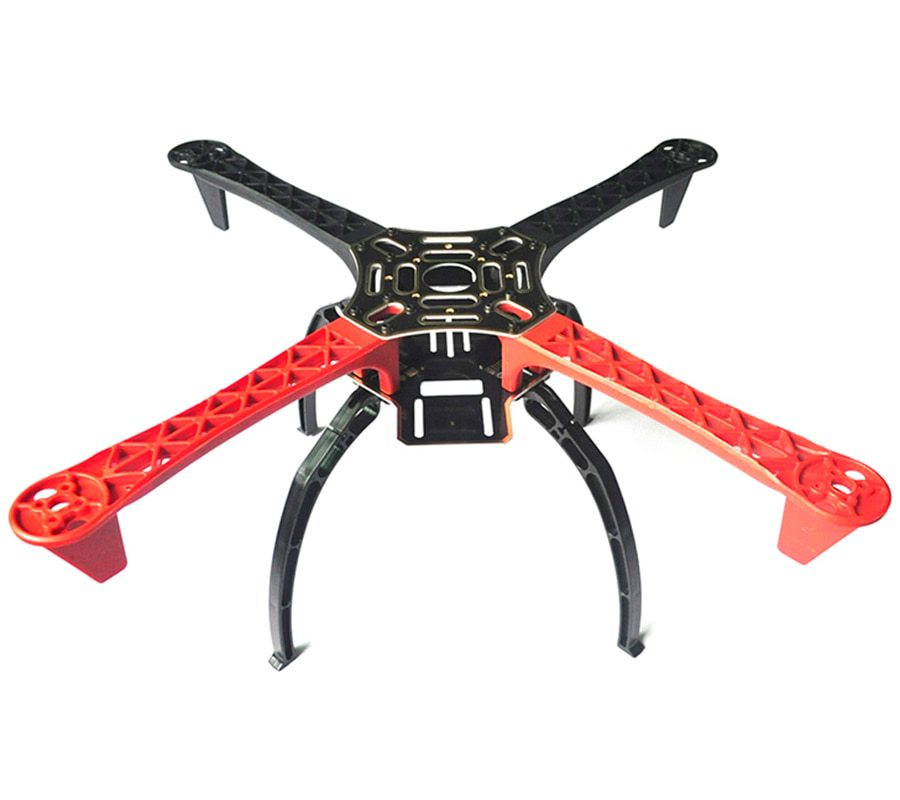
\includegraphics[scale=0.7]{figura2.jpg}
\caption{Telaio}
\label{figura2}
\end{figure}
\subsection{Motori con eliche ed ESC}
I motori montati sui droni (Figura 3) sono di tipo "Brushless". Essi funzionano senza bisogno di contatti elettrici striscianti sull'albero motore (ossia le "spazzole"), permettendo vantaggi come minor resistenza meccanica e peso inferiore. Necessitano però di un ulterior componente, l'ESC (Electronic Speed Controller).
\begin{figure}[!htpb]
\centering
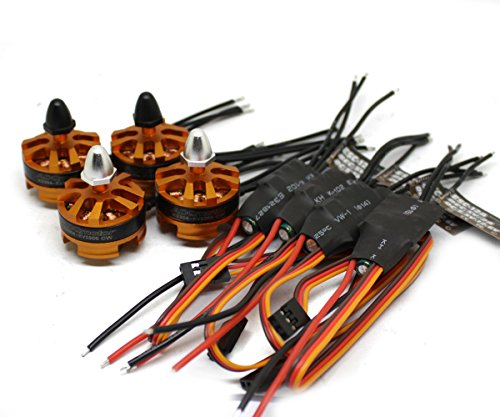
\includegraphics[scale=0.3]{figura3.jpg}
\caption{Motori}
\label{figura3}
\end{figure}
\subsection{Power Distribution Unit}
Centralina che permette la distribuzione di corrente dalla batteria ai 4 motori e alla board principale (Figura 4).
\begin{figure}[!htpb]
\centering
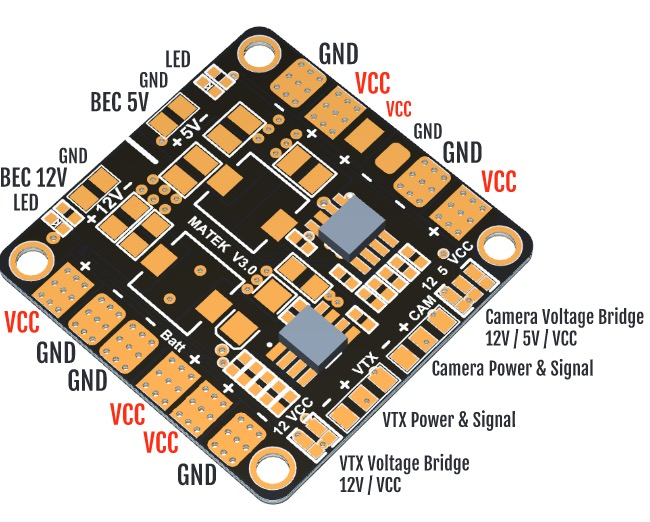
\includegraphics[scale=0.3]{figura4.png}
\caption{PDU}
\label{figura4}
\end{figure}
\subsection{Batteria Li-po}
\begin{figure}[!htpb]
\centering
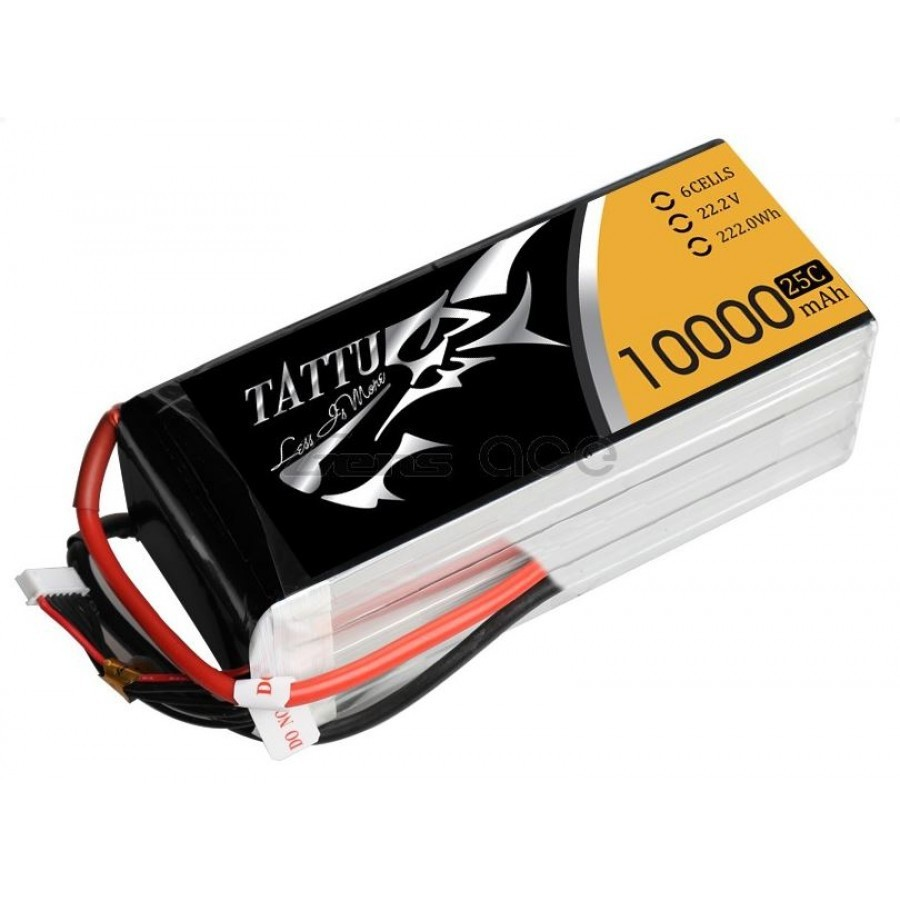
\includegraphics[scale=0.2]{figura5.jpg}
\caption{Batteria Li-Po}
\label{figura5}
\end{figure}
La batteria (Figura 5) deve essere leggera e molto capiente. Andrà ad alimentare motori e board principale. Da definire un sistema che determini il lvello di batteria, per capire quando si sta per scaricare (Led?).
\subsection{Giroscopio e Accelerometro} 
Componente essenziale per definire la corretta stabilità del drone.
\begin{figure}[!htpb]
\centering
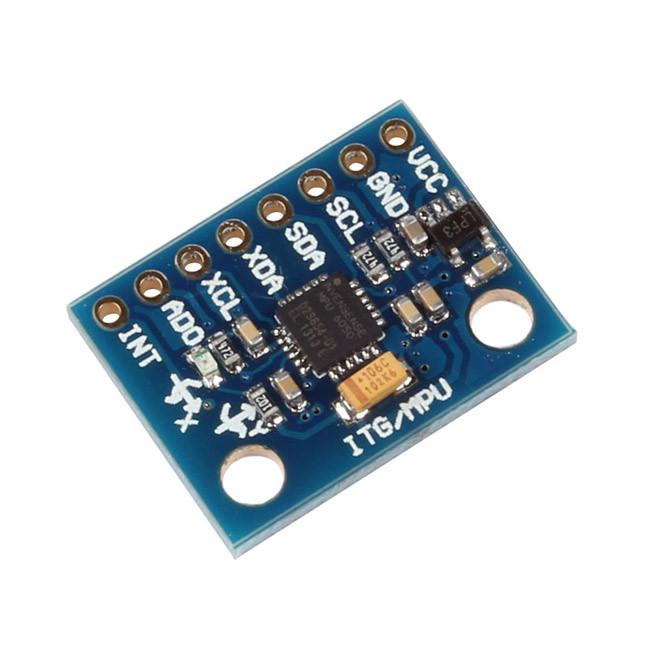
\includegraphics[scale=0.2]{figura6.jpg}
\caption{Giroscopio e Accelerometro}
\label{figura6}
\end{figure}
\section{Progetti esistenti}
Ovviamente i progetti già esistenti online sono numerosi, ma pochi sono i droni che hanno un volo molto preciso e stabile. Il progetto, a mio parere, migliore è quello realizzato da Joop Brokking. Infatti, oltre ad aver realizzato un drone telecomandato con una stabilità di volo perfetta, ha anche realizzato una guida completa tramite sito web e youtube dove spiega il funzionamento di ogni singolo componente nei dettagli, spiegando anche leggi fisiche e matematiche che ne derivano. Inoltre, spesso nei suoi progetti utilizza un semplice Arduino Uno.\\Sito web: \url{http://brokking.net/ymfc-al_main.html}\\Video esempio: \url{https://www.youtube.com/watch?v=gz-Mywo7bGc}\\
Una volta realizzato un drone simile, si potranno aggiungere le più svariate funzionalità, come il return to launch, dove il drone atterra esattamente nel punto in cui è decollato (\url{https://www.youtube.com/watch?v=1nnNfG6sAcs}), oppure come l'Obstacle avoiding, dove durante il volo esso sarà in grado di rilevare ostacoli (e potenzialmente eseguire una mappatura dell'ambiente)(\url{https://www.youtube.com/watch?v=mu--YnlI-dM}) 
\section{Note}
Essendomi appassionato al mondo dei Sistemi Embedded e dell'IOT, spero tramite questo tirocinio (e tesi), di imparare a risolvere i problemi di implementazione e realizzazione di progetti abbastanza complessi come questo, dove l'insieme di hardware e software deve interagire con forze esterne e imprevedibili.\\
Ovviamente, sono ben accette altre proposte che ritiene più interessanti.
\end{document}